\chapter{Elektronische spectroscopie en fotofysica}\label{ch:b3:electronic-spectroscopy}

Onder de ultravioletlamp van een donkere bar gloeit een glas tonic
bleekblauw, als een spook. Het kinine dat erin zit, absorbeert
ultraviolet licht, dat het oog niet kan zien, en geeft een deel ervan
enkele nanoseconden later terug als zichtbaar blauw licht. Absorptie, een
kort leven in een aangeslagen toestand, emissie bij een langere
golflengte, de energie die niet als licht terugkomt: het lot van een
aangeslagen molecuul is een wedstrijd tussen processen met
snelheidsconstanten, en zijn spectrum wordt gevormd door de vibraties van
het molecuul en door de symmetrieregels van
\cref{ch:b3:group-theory-applied}. Dit hoofdstuk bestudeert elektronische
overgangen en wat er daarna gebeurt, het domein van de fotofysica;
\cref{ch:b3:photochemistry} voegt de gevallen toe waarin het aangeslagen
molecuul reageert.

\begin{recall}
Het deel van jaar~1 mat absorbantie met de wet van Lambert-Beer, $A =
\varepsilon\ell c$, definieerde de molaire absorptiecoëfficiënt,
chromoforen en geconjugeerde systemen, en verbond kleur met het
absorptiemaximum. Het deel van jaar~2
benoemde de grensorbitalen HOMO en LUMO. \Cref{ch:b3:many-electron-atoms}
definieerde singulet- en \omterm{def:b3:many-electron-atoms:singlet-triplet}{triplettoestanden}; \cref{ch:b3:group-theory-applied} de
stelling over integralen die nul zijn; \cref{ch:b3:rovibrational-spectroscopy} de
vibratieniveaus van een binding.
\end{recall}

\begin{omfigure}
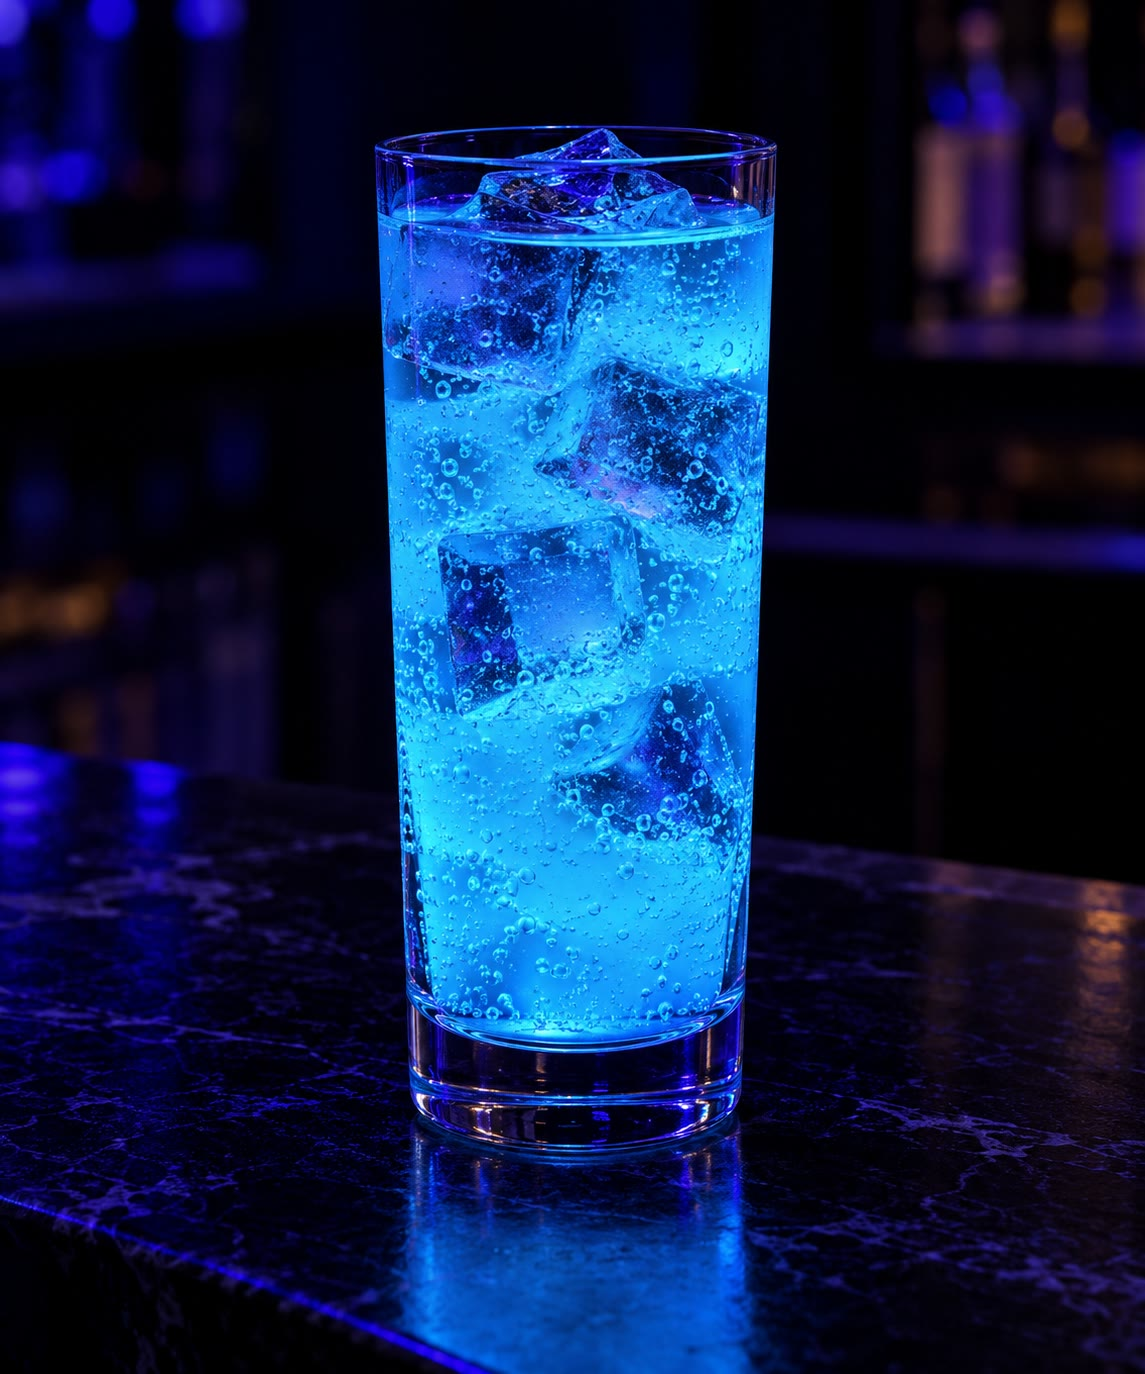
\includegraphics[height=4.6cm]{images/book4/ai/b3-07-tonic.jpg}\hspace{1em}%
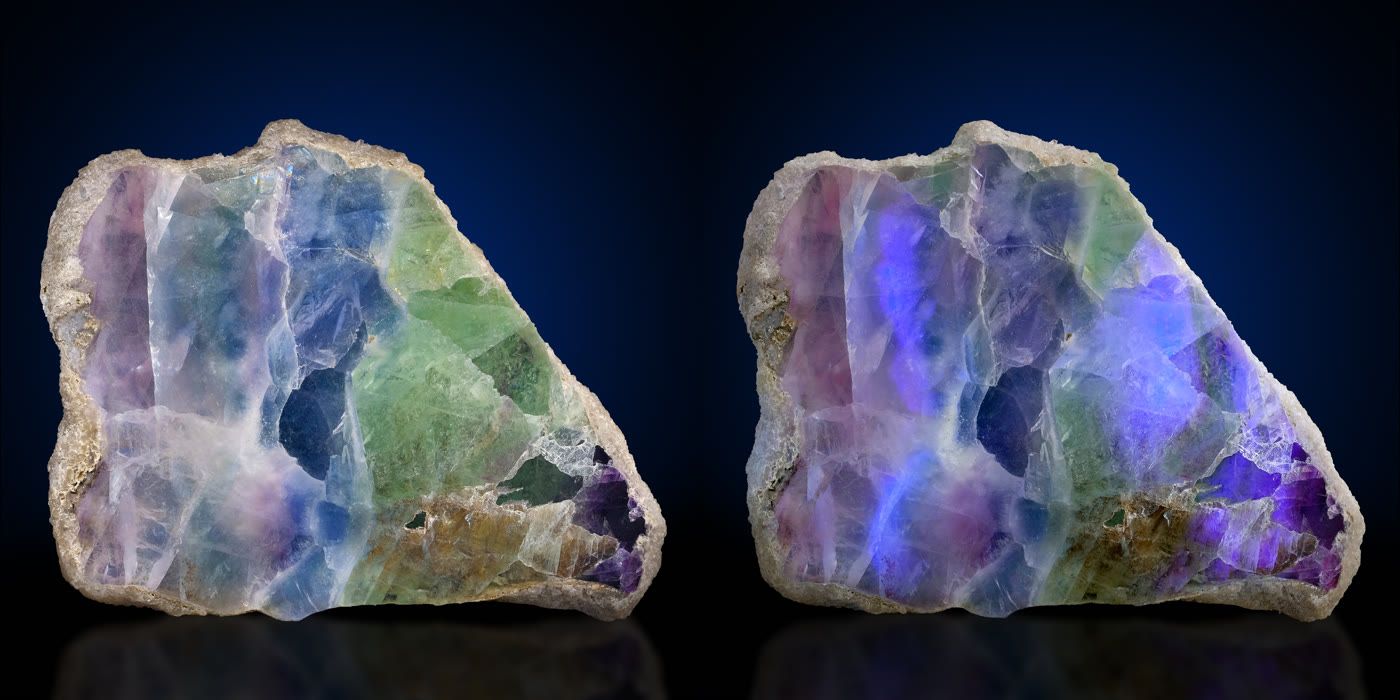
\includegraphics[height=4.6cm]{images/book4/fluorite-uv.jpg}

{\small Links: tonic die blauw oplicht onder een ultravioletlamp. Rechts:
fluoriet bij daglicht en fluorescerend onder ultraviolet licht; het
mineraal gaf de \omterm{def:b3:electronic-spectroscopy:luminescence}{fluorescentie} haar naam. Foto Masha Milshina, CC BY 4.0.}
\end{omfigure}

\section{Elektronische overgangen en hun selectieregels}

\begin{definition}[Overgangsdipoolmoment, oscillatorsterkte]\label{def:b3:electronic-spectroscopy:transition-dipole}
Het \emph{overgangsdipoolmoment}\index{overgangsdipoolmoment} tussen de
toestanden $\Psi_i$ en $\Psi_f$ is $\boldsymbol\mu_{fi} = \langle\Psi_f|\hat{\boldsymbol\mu}|\Psi_i
\rangle$, met $\hat{\boldsymbol\mu} = -e\sum_k\mathbf r_k$ (plus de
kernladingen, die tussen orthogonale toestanden wegvallen). De
\emph{oscillatorsterkte}\index{oscillatorsterkte} $f$ is de dimensieloze
maat voor de intensiteit van een band, ongeveer 1 voor de sterkste
overgangen.
\end{definition}

\begin{proposition}[Intensiteit en oscillatorsterkte]\label{prop:b3:electronic-spectroscopy:intensity}
De geïntegreerde absorptie van een band is evenredig met $|\boldsymbol\mu_{fi}|^2$,
en in de praktijk is
\[
f \approx 4.32\times10^{-9}\int\varepsilon(\tilde\nu)\,\dd\tilde\nu,
\]
met $\varepsilon$ in \unit{L.mol^{-1}.cm^{-1}} en $\tilde\nu$ in \unit{cm^{-1}}.
\end{proposition}
\admitted

De evenredigheid volgt uit de tijdsafhankelijke storingstheorie en de
numerieke factor uit de klassieke oscillator; beide horen thuis in meer
gevorderde cursussen. Wat hier telt, is dat $f$ alleen groot is als
$\boldsymbol\mu_{fi}$ dat is, en dat symmetrie het tot nul kan dwingen.

\begin{theorem}[De spinselectieregel]\label{thm:b3:electronic-spectroscopy:spin-rule}
Een elektrische-dipoolovergang tussen toestanden met verschillende totale
spin is verboden: $\Delta S = 0$.
\end{theorem}

\begin{proof}
Elke toestand is een product van een ruimtelijke functie en een
spinfunctie, $\Psi = \phi\,\chi$.
De dipooloperator werkt alleen op de posities in, dus $\langle\phi_f\chi_f|\hat{\boldsymbol\mu}|
\phi_i\chi_i\rangle = \langle\phi_f|\hat{\boldsymbol\mu}|\phi_i\rangle\langle\chi_f|\chi_i\rangle$.
Spinfuncties met verschillende $S$ zijn \omterm{def:b3:quantum-model-systems:operator}{eigenfuncties} van $\hat S^2$ met
verschillende \omterm{def:b3:quantum-model-systems:operator}{eigenwaarden}, en dus orthogonaal (\cref{thm:b3:quantum-model-systems:hermitian-real}):
de tweede factor is nul.
\end{proof}

\begin{theorem}[De regel van Laporte]\label{thm:b3:electronic-spectroscopy:laporte}
In een molecuul met een \omterm{def:b3:point-groups:inversion}{inversiecentrum} moet een elektrische-dipoolovergang
van pariteit veranderen: $g \leftrightarrow u$ is toegestaan, $g \leftrightarrow g$ en $u
\leftrightarrow u$ zijn verboden. Dit is de
\emph{regel van Laporte}\index{regel van Laporte}.
\end{theorem}

\begin{proof}
De componenten van $\hat{\boldsymbol\mu}$ veranderen van teken onder
inversie: ze zijn $u$.
Het product $\Gamma_f\otimes\Gamma_\mu\otimes\Gamma_i$ is alleen $g$ als $\Gamma_f$ en $\Gamma_i$
tegengestelde pariteiten hebben; anders is het $u$ en kan het de
\omterm{def:b3:group-theory-applied:reducible}{totaalsymmetrische representatie} niet bevatten
(\cref{thm:b3:group-theory-applied:vanishing-integral}).
\end{proof}

De twee regels zijn strikt voor de geïdealiseerde toestanden; echte
moleculen versoepelen ze --- \omterm{def:b3:many-electron-atoms:spin-orbit}{spin-baankoppeling} mengt singulet- en
tripletkarakter, vibraties heffen het symmetriecentrum even op --- en de
``verboden'' overgangen verschijnen, zwak. De $d$--$d$-banden van
octaëdrische complexen, verboden volgens Laporte en zwak, danken hun
kleur aan deze versoepeling
(\cref{ch:b3:complex-spectra-magnetism}).

\begin{definition}[Ladingsoverdrachtsovergang]\label{def:b3:electronic-spectroscopy:charge-transfer}
Een \emph{ladingsoverdrachtsovergang}\index{ladingsoverdrachtsovergang}
brengt een elektron over van een orbitaal die vooral op één deel van een
systeem gelokaliseerd is (een donor) naar een orbitaal die vooral op een
ander deel gelokaliseerd is (een acceptor); haar overgangsdipool is groot,
haar band intens en breed, en haar energie gevoelig voor de polariteit
van het oplosmiddel.
\end{definition}

\begin{method}[Een absorptieband toekennen]\label{met:b3:electronic-spectroscopy:assign-band}
\begin{enumerate}
  \item $\varepsilon_{\max}$ boven ongeveer \qty{e4}{L.mol^{-1}.cm^{-1}}: een toegestane
        overgang ($\pi\to\pi^*$ van een geconjugeerd systeem, of
        ladingsoverdracht).
  \item $\varepsilon_{\max}$ van 10 tot enkele honderden: een verboden overgang ($n\to\pi^*$,
        symmetrieverboden; $d$--$d$, verboden volgens Laporte).
  \item $\varepsilon_{\max}$ onder 1: spinverboden.
  \item Een $n\to\pi^*$-band verschuift in protische oplosmiddelen naar
        kortere golflengten (het vrije elektronenpaar wordt door
        waterstofbruggen gestabiliseerd), een $\pi\to\pi^*$-band meestal
        naar langere.
\end{enumerate}
\end{method}

\section{Het franck-condonprincipe}

\begin{theorem}[Franck-condonprincipe]\label{thm:b3:electronic-spectroscopy:franck-condon}
Binnen de \omterm{def:b3:computational-chemistry:born-oppenheimer}{born-oppenheimerbenadering}, en als de overgangsdipool weinig
afhangt van de kernposities, is de intensiteit van de \omterm{def:b3:electronic-spectroscopy:vibronic}{vibronische
overgang} van vibratieniveau $v''$ van de lagere elektronische toestand
naar niveau $v'$ van de hogere evenredig met $|\langle\chi_{v'}|\chi_{v''}\rangle|^2$, het
kwadraat van de overlap van de twee vibratiegolffuncties: dit is het
\emph{franck-condonprincipe}\index{franck-condonprincipe}. Elektronische
overgangen zijn verticaal: de kernen bewegen niet terwijl de elektronen
springen.
\end{theorem}

\begin{proof}
Met $\Psi = \psi_{\mathrm{el}}(\mathbf r;R)\chi_v(R)$ is het overgangsmoment
$\int\chi_{v'}^*\big[\int\psi'^*_{\mathrm{el}}\hat\mu\psi''_{\mathrm{el}}\dd\mathbf r\big]
\chi_{v''}\,\dd R$. De uitdrukking tussen haken is het elektronische
overgangsmoment
$\mu_{\mathrm{el}}(R)$; als constant beschouwd (de condonbenadering)
komt het buiten
de integraal, en er blijft $\mu_{\mathrm{el}}\langle\chi_{v'}|\chi_{v''}\rangle$ over.
\end{proof}

\begin{definition}[Vibronische overgang, progressie, franck-condonfactor]\label{def:b3:electronic-spectroscopy:vibronic}
Een \emph{vibronische overgang}\index{vibronische overgang} verandert de
elektronische en de vibratietoestand tegelijk; de lijnen $v' \leftarrow 0$ voor $v' = 0, 1, 2,
\dots$ vormen een \emph{vibronische progressie}\index{vibronische progressie}; de
\emph{franck-condonfactor}\index{franck-condonfactor} van een vibronische
lijn is
$|\langle\chi_{v'}|\chi_{v''}\rangle|^2$.
\end{definition}

\begin{proposition}[Verschoven oscillatoren]\label{prop:b3:electronic-spectroscopy:displaced}
Als beide toestanden harmonisch zijn met dezelfde frequentie en het
minimum van de hogere toestand verschoven is over $\Delta$ (in eenheden van
$\sqrt{\hbar/m\omega}$), vormen de \omterm{def:b3:electronic-spectroscopy:vibronic}{franck-condonfactoren} vanuit $v'' = 0$
een poissonverdeling,
$|\langle v'|0\rangle|^2 = \eu^{-S}S^{v'}/v'!$, met $S = \Delta^2/2$; de sterkste
lijn ligt bij ongeveer $v' = S$.
\end{proposition}
\admitted

Het algemene bewijs gebruikt de \omterm{def:b3:quantum-model-systems:ladder}{ladderoperatoren} van
\cref{ch:b3:quantum-model-systems}; de figuurgegevens van dit hoofdstuk
toetsen de formule aan een directe integratie. Een kleine verschuiving
geeft één sterke 0--0-lijn; een grote een lange progressie waarvan het
sterkste lid ver van de 0--0-lijn ligt.

\begin{omfigure}
\begin{tikzpicture}
\begin{axis}[name=pc, width=0.46\linewidth, height=6cm, xmin=-4, xmax=5, ymin=0,
  ymax=14, axis lines=left, xtick=\empty, ytick=\empty, xlabel={kerncoördinaat},
  ylabel={energie}, label style={font=\small}]
\addplot[black, thick] table[x=y, y=ground] {figdata/out/bachelor-3-franck-condon-curves.dat};
\addplot[omDef, thick] table[x=y, y=excited] {figdata/out/bachelor-3-franck-condon-curves.dat};
\draw[omabs] (axis cs:0,0.5) -- (axis cs:0,10.6);
\draw[omvib] (axis cs:-1,0.5) -- (axis cs:1,0.5);
\draw[omvib] (axis cs:0.732,9.5) -- (axis cs:2.732,9.5);
\draw[omvib] (axis cs:-0.000,10.5) -- (axis cs:3.464,10.5);
\draw[omvib] (axis cs:-0.504,11.5) -- (axis cs:3.968,11.5);
\draw[omvib] (axis cs:-0.914,12.5) -- (axis cs:4.378,12.5);
\node[font=\small, anchor=west] at (axis cs:-3.9,12.0) {aangeslagen};
\node[font=\small, anchor=south east] at (axis cs:4.95,0.1) {grondtoestand};
\node[font=\scriptsize, anchor=east] at (axis cs:-0.05,5.5) {verticaal};
\end{axis}
\begin{axis}[at={(pc.east)}, anchor=west, xshift=1.3cm, width=0.46\linewidth,
  height=6cm, xmin=-0.5, xmax=12.5, ymin=0, ymax=0.8, axis lines=left, ycomb,
  xlabel={$v'$}, ylabel={franck-condonfactor}, label style={font=\small},
  tick label style={font=\small}]
\addplot[black, very thick] table[x=v, y=s03] {figdata/out/bachelor-3-franck-condon-sticks.dat};
\addplot[omDef, very thick, xshift=2pt] table[x=v, y=s15] {figdata/out/bachelor-3-franck-condon-sticks.dat};
\addplot[omThm, very thick, xshift=4pt] table[x=v, y=s5] {figdata/out/bachelor-3-franck-condon-sticks.dat};
\end{axis}
\end{tikzpicture}

{\small Links: een verticale overgang vanuit het laagste niveau van de
grondtoestand belandt waar de kromme van de aangeslagen toestand, verschoven naar een
grotere bindingslengte, hoog boven haar minimum ligt (getekend voor $S = 1.5$).
Rechts: \omterm{def:b3:electronic-spectroscopy:vibronic}{franck-condonfactoren} van de progressie voor $S = 0.3$ (zwart), 1.5
(blauw) en 5 (rood); elke reeks telt op tot 1.}
\end{omfigure}

\begin{example}[Jood]\label{ex:b3:electronic-spectroscopy:iodine}
% ledger: diat:I2.re, diat:I2B.re, diat:I2B.we, imass:I127
Jooddamp is violet omdat zijn band B$\leftarrow$X geelgroen licht absorbeert.
De binding verlengt van \qty{266.6}{pm} in de grondtoestand tot \qty{302.5}{pm} in
de toestand B. In het model van de verschoven oscillatoren met de
frequentie van de toestand B
(\qty{125.7}{cm^{-1}}) geeft $\Delta R = \qty{35.8}{pm}$ de waarde $S \approx 15$: de absorptie is een
lange progressie waarvan de sterkste lijnen eindigen op hoge
vibratieniveaus van de toestand B, en waarvan het vervolg overgaat in het
dissociatiecontinuüm.
\end{example}

\section{Het lot van een aangeslagen toestand: het jablonskidiagram}

\begin{definition}[Jablonskidiagram]\label{def:b3:electronic-spectroscopy:jablonski}
Een \emph{jablonskidiagram}\index{jablonskidiagram} toont de elektronische
toestanden van een molecuul (singuletten $S_0, S_1, S_2, \dots$ in één kolom,
tripletten $T_1, T_2,
\dots$ in een andere), hun vibratieniveaus, en de processen die ze
verbinden: stralingsprocessen als rechte pijlen, stralingsloze als
golvende pijlen.
\end{definition}

\begin{definition}[Stralingsloze processen]\label{def:b3:electronic-spectroscopy:radiationless}
\emph{Vibratierelaxatie}\index{vibratierelaxatie} brengt een aangeslagen
molecuul door botsingen in enkele picoseconden naar het laagste
vibratieniveau van zijn elektronische toestand.
\emph{Interne conversie}\index{interne conversie}
is een stralingsloze overgang tussen toestanden met dezelfde
multipliciteit ($S_2 \to S_1$, $S_1 \to S_0$); \emph{intersystem
crossing}\index{intersystem crossing} is er een tussen toestanden met
verschillende multipliciteit ($S_1 \to T_1$, $T_1 \to S_0$).
\end{definition}

\begin{definition}[Luminescentie, fluorescentie, fosforescentie, stokesverschuiving]\label{def:b3:electronic-spectroscopy:luminescence}
\emph{Luminescentie}\index{luminescentie} is de uitzending van licht door
een aangeslagen molecuul. \emph{Fluorescentie}\index{fluorescentie} is
spintoegestane emissie, meestal $S_1 \to S_0$, snel (nanoseconden);
\emph{fosforescentie}\index{fosforescentie}
is spinverboden emissie, meestal $T_1 \to S_0$, traag (milliseconden tot
seconden). De \emph{stokesverschuiving}\index{stokesverschuiving} is het
verschil tussen het absorptie- en het emissiemaximum, in energie.
\end{definition}

\begin{omfigure}
\begin{tikzpicture}[font=\small, >=Stealth]
  \foreach \y/\l in {0/{$S_0$}, 3.4/{$S_1$}, 5.6/{$S_2$}}{
    \draw[omstate] (0,\y) -- (3.6,\y); \node[anchor=east] at (-0.1,\y) {\l};
    \foreach \d in {0.25,0.5,0.75}{\draw[omvib] (0,\y+\d) -- (3.6,\y+\d);}}
  \draw[omstate] (5.0,2.5) -- (7.6,2.5); \node[anchor=west] at (7.7,2.5) {$T_1$};
  \foreach \d in {0.25,0.5,0.75}{\draw[omvib] (5.0,2.5+\d) -- (7.6,2.5+\d);}
  \draw[omabs] (0.3,0) -- (0.3,4.15) node[pos=0.35, left, font=\scriptsize, align=right] {absorptie};
  \draw[omabs] (0.7,0) -- (0.7,5.85);
  \draw[omnonrad] (1.05,5.85) -- (1.05,5.6);
  \draw[omnonrad] (1.05,5.6) -- (1.05,3.4) node[pos=0.5, right, font=\scriptsize] {IC};
  \draw[omnonrad] (0.45,4.15) -- (0.45,3.42);
  \draw[omfluo] (1.7,3.4) -- (1.7,0.5) node[pos=0.5, right, font=\scriptsize, align=left] {fluores-\\centie};
  \draw[omnonrad] (3.2,3.4) -- (3.2,0.02) node[pos=0.5, right, font=\scriptsize] {IC};
  \draw[omisc] (3.6,3.4) -- (5.0,3.1) node[pos=0.5, above, font=\scriptsize] {ISC};
  \draw[omnonrad] (5.3,3.1) -- (5.3,2.52);
  \draw[omphos] (6.0,2.5) -- (6.0,0.5) node[pos=0.5, right, font=\scriptsize, align=left] {fosfores-\\centie};
  \draw[omisc] (5.6,2.5) -- (3.7,0.02) node[pos=0.45, above left, font=\scriptsize, inner sep=1pt] {ISC};
  \draw[omvib, dashed] (3.6,0.5) -- (6.0,0.5);
  \draw[omvib, dashed] (3.6,0.0) -- (7.6,0.0);
\end{tikzpicture}

{\small Een \omterm{def:b3:electronic-spectroscopy:jablonski}{jablonskidiagram}. Rechte pijlen: absorptie (blauw),
\omterm{def:b3:electronic-spectroscopy:luminescence}{fluorescentie} (rood), \omterm{def:b3:electronic-spectroscopy:luminescence}{fosforescentie} (oranje); golvende pijlen:
\omterm{def:b3:electronic-spectroscopy:radiationless}{vibratierelaxatie} en \omterm{def:b3:electronic-spectroscopy:radiationless}{interne conversie} (IC); gestreepte golvende pijlen:
\omterm{def:b3:electronic-spectroscopy:radiationless}{intersystem crossing} (ISC).
De emissie vertrekt vanuit het laagste vibratieniveau van $S_1$ of $T_1$
en kan eindigen op elk niveau van $S_0$.}
\end{omfigure}

\begin{proposition}[Regel van Kasha]\label{prop:b3:electronic-spectroscopy:kasha}
\omterm{def:b3:electronic-spectroscopy:luminescence}{Luminescentie} treedt, op zeer weinig uitzonderingen na, op vanuit de
laagste aangeslagen toestand van een gegeven multipliciteit ($S_1$ of $T_1$),
welke toestand er ook eerst aangeslagen werd: de
\emph{regel van Kasha}\index{regel van Kasha}.
\end{proposition}
\begin{proof}[Status]
Experimenteel vastgesteld; de reden is dat \omterm{def:b3:electronic-spectroscopy:radiationless}{interne conversie} tussen de
hogere aangeslagen toestanden, die dicht bij elkaar liggen, veel sneller
is dan emissie, terwijl de afstand $S_1$--$S_0$ groot is.
\end{proof}

\begin{proposition}[Spiegelbeeld]\label{prop:b3:electronic-spectroscopy:mirror}
Als de aangeslagen toestand en de grondtoestand een gelijkaardige
vibratiestructuur hebben, is de fluorescentieband het spiegelbeeld van
de eerste absorptieband ten opzichte van hun gemeenschappelijke
0--0-lijn; de emissie ligt bij langere golflengten (\omterm{def:b3:electronic-spectroscopy:luminescence}{stokesverschuiving}).
\end{proposition}

\begin{proof}
Absorptie gaat van $v'' = 0$ naar de niveaus $v'$ van $S_1$, bij $E_{00} + v'h\nu'$; emissie
van $v' = 0$ naar de niveaus $v''$ van $S_0$, bij $E_{00} - v''h\nu''$. Met
gelijke frequenties en dezelfde \omterm{def:b3:electronic-spectroscopy:vibronic}{franck-condonfactoren} (gelijke
verschuiving) liggen de twee progressies symmetrisch ten opzichte van $E_{00}$.
\end{proof}

\begin{omfigure}
\begin{tikzpicture}
\begin{axis}[width=0.75\linewidth, height=5cm, xmin=17, xmax=33, ymin=0,
  ymax=1.15, axis x line=bottom, axis y line=left, ytick=\empty,
  xlabel={golfgetal / $10^3$ cm$^{-1}$}, ylabel={intensiteit},
  legend cell align=left, legend style={font=\small, draw=none, at={(0.02,0.97)}, anchor=north west},
  tick label style={font=\small}, label style={font=\small}]
\addplot[omDef, thick] table[x=nu, y=abs] {figdata/out/bachelor-3-photophysics-bands.dat};
\addlegendentry{absorptie}
\addplot[omThm, thick] table[x=nu, y=em] {figdata/out/bachelor-3-photophysics-bands.dat};
\addlegendentry{fluorescentie}
\draw[gray, dashed] (axis cs:25,0) -- (axis cs:25,1.12);
\node[font=\scriptsize, gray, anchor=south west] at (axis cs:25,1.0) {0--0};
\end{axis}
\end{tikzpicture}

{\small Absorptie en \omterm{def:b3:electronic-spectroscopy:luminescence}{fluorescentie} van een modelmolecuul ($S = 1$,
vibratiekwantum \qty{1400}{cm^{-1}}): spiegelbeelden ten opzichte van de
0--0-lijn; de maxima liggen uit elkaar volgens de \omterm{def:b3:electronic-spectroscopy:luminescence}{stokesverschuiving}.}
\end{omfigure}

\section{Kinetiek van aangeslagen toestanden}

Na de excitatie neemt de bezetting van $S_1$ af via elk proces dat
daarvoor openstaat, elk van de eerste orde: stralingsverval $k_r$, \omterm{def:b3:electronic-spectroscopy:radiationless}{interne
conversie} $k_{\mathrm{IC}}$,
\omterm{def:b3:electronic-spectroscopy:radiationless}{intersystem crossing} $k_{\mathrm{ISC}}$.

\begin{definition}[Levensduur van de aangeslagen toestand, stralingslevensduur]\label{def:b3:electronic-spectroscopy:lifetime}
De \emph{levensduur van de aangeslagen toestand}\index{levensduur van de aangeslagen toestand} is $\tau =
1/\sum k$, de tijdconstante van het exponentiële verval van de aangeslagen
bezetting. De \emph{stralingslevensduur}\index{stralingslevensduur} $\tau_r =
1/k_r$ is de levensduur die de toestand zou hebben als emissie zijn
enige lot was.
\end{definition}

\begin{definition}[Kwantumopbrengst]\label{def:b3:electronic-spectroscopy:quantum-yield}
De \emph{kwantumopbrengst}\index{kwantumopbrengst} van een proces dat
volgt op de absorptie van licht, is het aantal gebeurtenissen van dat
proces gedeeld door het aantal geabsorbeerde fotonen. De
\emph{kwantumopbrengst van
fluorescentie}\index{kwantumopbrengst van fluorescentie} $\Phi_F$ is het
aantal fotonen dat als \omterm{def:b3:electronic-spectroscopy:luminescence}{fluorescentie} uitgezonden wordt per geabsorbeerd
foton.
\end{definition}

\begin{proposition}[Kwantumopbrengst en levensduur]\label{prop:b3:electronic-spectroscopy:quantum-yield}
$\Phi_F = k_r/(k_r + k_{\mathrm{IC}} + k_{\mathrm{ISC}}) = k_r\tau = \tau/\tau_r$; op dezelfde
manier is
$\Phi_{\mathrm{ISC}} = k_{\mathrm{ISC}}\tau$, en de opbrengsten van de
concurrerende processen tellen op tot 1.
\end{proposition}

\begin{proof}
$\dd[S_1]/\dd t = -(k_r + k_{\mathrm{IC}} + k_{\mathrm{ISC}})[S_1]$, dus $[S_1] = [S_1]_0\eu^{-t/\tau}$.
Het aantal uitgezonden fotonen is $\int_0^\infty k_r[S_1]\,\dd t = k_r\tau[S_1]_0$, op
$[S_1]_0$ aangeslagen moleculen. Dezelfde integraal met elke $k$ geeft
elke opbrengst,
en hun som is $\tau\sum k = 1$.
\end{proof}

\begin{definition}[Fluorescentiedover, dynamische en statische uitdoving]\label{def:b3:electronic-spectroscopy:quencher}
Een \emph{fluorescentiedover}\index{fluorescentiedover} is een deeltje dat
de \omterm{def:b3:electronic-spectroscopy:luminescence}{fluorescentie} vermindert. Bij \emph{dynamische
uitdoving}\index{dynamische uitdoving} deactiveert het het aangeslagen
molecuul bij een botsing, wat een snelheid $k_q[Q]$ toevoegt en de
levensduur verkort; bij \emph{statische uitdoving}\index{statische uitdoving}
vormt het een niet-fluorescerend complex met het molecuul in de
grondtoestand, wat de intensiteit vermindert zonder de levensduur te
veranderen van de moleculen die nog uitzenden.
\end{definition}

\begin{theorem}[Vergelijking van Stern-Volmer]\label{thm:b3:electronic-spectroscopy:stern-volmer}
Voor \omterm{def:b3:electronic-spectroscopy:quencher}{dynamische uitdoving} geldt
\[
\frac{I_0}{I} = \frac{\tau_0}{\tau} = 1 + k_q\tau_0[Q] = 1 + K_{SV}[Q],
\]
de \emph{vergelijking van Stern-Volmer}\index{vergelijking van Stern-Volmer}, waarin $I_0$, $\tau_0$
zonder dover gemeten worden en $K_{SV} = k_q\tau_0$.
\end{theorem}

\begin{proof}
Met dover is $\tau = 1/(k_0 + k_q[Q])$ met $k_0 = 1/\tau_0$, dus $\tau_0/\tau = 1 +
k_q\tau_0[Q]$. De intensiteit is evenredig met $\Phi_F = k_r\tau$, dus $I_0/I = \tau_0/\tau$.
\end{proof}

\begin{omfigure}
\begin{tikzpicture}
\begin{axis}[name=dec, width=0.5\linewidth, height=5cm, xmin=0, xmax=40, ymode=log,
  ymin=0.005, ymax=1.2, axis lines=left, xlabel={$t$ / ns}, ylabel={$I(t)/I(0)$},
  legend cell align=left, legend style={font=\scriptsize, draw=none, at={(0.98,0.98)}, anchor=north east},
  tick label style={font=\small}, label style={font=\small}]
\addplot[black, thick] table[x=t, y=q0] {figdata/out/bachelor-3-photophysics-decays.dat};
\addlegendentry{$[Q] = 0$}
\addplot[omDef, thick] table[x=t, y=q1] {figdata/out/bachelor-3-photophysics-decays.dat};
\addlegendentry{0.01 M}
\addplot[omProp, thick] table[x=t, y=q2] {figdata/out/bachelor-3-photophysics-decays.dat};
\addlegendentry{0.02 M}
\addplot[omThm, thick] table[x=t, y=q4] {figdata/out/bachelor-3-photophysics-decays.dat};
\addlegendentry{0.04 M}
\end{axis}
\begin{axis}[at={(dec.east)}, anchor=west, xshift=1.4cm, width=0.42\linewidth,
  height=5cm, xmin=0, xmax=0.045, ymin=0, ymax=3.3, axis lines=left,
  xlabel={$[Q]$ / mol L$^{-1}$}, ylabel={$I_0/I = \tau_0/\tau$},
  xticklabel style={/pgf/number format/fixed, /pgf/number format/precision=2},
  scaled x ticks=false, tick label style={font=\small}, label style={font=\small}]
\addplot[omThm, thick, mark=*] table[x=Q, y=I0I] {figdata/out/bachelor-3-photophysics-sv.dat};
\end{axis}
\end{tikzpicture}

{\small \omterm{def:b3:electronic-spectroscopy:quencher}{Dynamische uitdoving} van een modelfluorofoor ($\tau_0 = \qty{10}{ns}$, $k_q =
\qty{5e9}{L.mol^{-1}.s^{-1}}$). Links: fluorescentieverval, rechte lijnen op
een logaritmische schaal, steiler naarmate er meer dover is. Rechts: de
rechte van Stern-Volmer, met helling
$K_{SV} = k_q\tau_0 = \qty{50}{L/mol}$.}
\end{omfigure}

\begin{method}[Relatieve kwantumopbrengst van fluorescentie]\label{met:b3:electronic-spectroscopy:relative-yield}
\begin{enumerate}
  \item Kies een standaard met bekende $\Phi_{\mathrm{std}}$ die bij dezelfde
        excitatiegolflengte absorbeert.
  \item Maak verdunde oplossingen ($A < 0.1$, om heropname te vermijden) en
        meet hun absorbanties $A$ en geïntegreerde emissiespectra $F$
        onder identieke omstandigheden.
  \item $\Phi = \Phi_{\mathrm{std}}\,\dfrac{F}{F_{\mathrm{std}}}\,\dfrac{A_{\mathrm{std}}}{A}\,
        \dfrac{n^2}{n_{\mathrm{std}}^2}$, waarbij de laatste factor corrigeert
        voor de brekingsindices van de oplosmiddelen.
\end{enumerate}
\end{method}

\begin{method}[Uitdovingsgegevens analyseren]\label{met:b3:electronic-spectroscopy:stern-volmer}
\begin{enumerate}
  \item Zet $I_0/I$ uit tegen $[Q]$; een rechte door 1 geeft $K_{SV}$.
  \item Meet ook levensduren: als $\tau_0/\tau$ dezelfde rechte volgt, is de
        uitdoving dynamisch, en $k_q = K_{SV}/\tau_0$; als $\tau$ niet
        verandert, is ze statisch.
  \item Vergelijk $k_q$ met de diffusiegrens, ongeveer \qty{e10}{L.mol^{-1}.s^{-1}} in
        water (\cref{ch:b3:rate-theories}): een $k_q$ die er dicht bij ligt,
        betekent dat vrijwel elke ontmoeting uitdooft.
\end{enumerate}
\end{method}

\begin{example}[Kinine en antraceen]\label{ex:b3:electronic-spectroscopy:quinine}
% ledger: fl:quinine.labs, fl:quinine.eps, fl:quinine.phi, fl:anthracene.labs, fl:anthracene.phi
Kininesulfaat in \qty{0.5}{M} zwavelzuur absorbeert bij \qty{349}{nm} met $\varepsilon =
\qty{5700}{L.mol^{-1}.cm^{-1}}$ en fluoresceert met $\Phi_F = 0.546$, wat er de
klassieke standaard voor relatieve \omterm{def:b3:electronic-spectroscopy:quantum-yield}{kwantumopbrengsten} van maakt.
Antraceen in cyclohexaan
absorbeert bij \qty{356}{nm} en heeft $\Phi_F = 0.36$; de meeste overige
aangeslagen moleculen gaan over naar de triplet.
\end{example}

\section{Toepassingen}

\omterm{def:b3:electronic-spectroscopy:luminescence}{Fluorescentie} wordt gedetecteerd tegen een donkere achtergrond, wat
fluorimetrie honderd tot duizend keer gevoeliger maakt dan
absorptiespectroscopie: nanomolaire concentraties van een fluorescerende
verbinding worden routinematig gemeten. Fluorescente probes rapporteren
over hun omgeving via hun golflengte, opbrengst of levensduur (polariteit,
pH, de binding van een ion); energieoverdracht tussen twee fluoroforen,
alleen efficiënt over enkele nanometer, meet afstanden in eiwitten.
Fosforescerende complexen van zware metalen, waarin \omterm{def:b3:many-electron-atoms:spin-orbit}{spin-baankoppeling}
\omterm{def:b3:electronic-spectroscopy:radiationless}{intersystem crossing} efficiënt maakt, oogsten tripletten in de
lichtgevende diodes van beeldschermen.

\begin{inthelab}[Tijdgecorreleerde enkelvoudige-fotontelling]
Om een levensduur van enkele nanoseconden te meten, wordt het monster
aangeslagen door een gepulste laserdiode met een herhalingsfrequentie in
het megahertzbereik, en wordt bij elke puls de vertraging van het eerste
gedetecteerde fluorescentiefoton geregistreerd. Na miljoenen pulsen is het
histogram van de vertragingen de vervalkromme, waaruit $\tau$ aangepast
wordt, met de instrumentrespons gemeten op een verstrooiende oplossing.
De ultravioletbron is afgeschermd; de gebruiker werkt met een bril die
haar golflengte tegenhoudt.
\end{inthelab}

\begin{history}[Stokes, 1852]
George Gabriel Stokes stuurde zonlicht door een violet glas en een prisma
in een kinineoplossing, en zag blauw licht opkomen uit het gebied dat door
onzichtbare ultraviolette stralen belicht werd: het uitgezonden licht had
altijd een langere golflengte dan het geabsorbeerde. Hij noemde het
verschijnsel \omterm{def:b3:electronic-spectroscopy:luminescence}{fluorescentie}, naar het mineraal fluoriet, dat op dezelfde
manier oplicht.
\end{history}

\section{Oefeningen}

\begin{exercise}[$\star$]\label{exo:b3:electronic-spectroscopy:1}
Toegestaan of verboden, en volgens welke regel: (a) $S_0 \to T_1$ in benzeen; (b) een $d$--$d$-overgang
van een octaëdrisch complex; (c) de overgang $\pi\to\pi^*$ van etheen
($B_{1u} \leftarrow A_g$ in $D_{2h}$); (d) de overgang $n\to\pi^*$ van methanal
($A_2$)?
\end{exercise}

\begin{exercise}[$\star$]\label{exo:b3:electronic-spectroscopy:2}
Een verbinding absorbeert bij \qty{349}{nm} en fluoresceert met een maximum bij
\qty{450}{nm} (gegevens van de oefening). Bereken de \omterm{def:b3:electronic-spectroscopy:luminescence}{stokesverschuiving} in
\unit{cm^{-1}} en in
eV.
\end{exercise}

\begin{exercise}[$\star$]\label{exo:b3:electronic-spectroscopy:3}
% ledger: fl:quinine.eps
Bereken de absorbantie bij \qty{349}{nm} van een oplossing van kininesulfaat van
\qty{1.0e-5}{mol/L} in een cuvet van \qty{1}{cm}, en de fractie van het
licht die ze absorbeert.
\end{exercise}

\begin{exercise}[$\star$]\label{exo:b3:electronic-spectroscopy:4}
Een fluorofoor heeft $\Phi_F = 0.60$ en $\tau = \qty{4.0}{ns}$. Bereken $k_r$, de
\omterm{def:b3:electronic-spectroscopy:lifetime}{stralingslevensduur} en de som van de niet-stralende snelheidsconstanten.
\end{exercise}

\begin{exercise}[$\star\star$]\label{exo:b3:electronic-spectroscopy:5}
Een band is gaussvormig met $\varepsilon_{\max} = \qty{5700}{L.mol^{-1}.cm^{-1}}$ en een
volle breedte op halve hoogte van \qty{5000}{cm^{-1}}. Schat haar
\omterm{def:b3:electronic-spectroscopy:transition-dipole}{oscillatorsterkte} (de integraal van een gausskromme is
$1.0645\,\varepsilon_{\max}\times$FWHM).
\end{exercise}

\begin{exercise}[$\star\star$]\label{exo:b3:electronic-spectroscopy:6}
Bepaal voor verschoven oscillatoren de sterkste lijn van de progressie
voor $S = 0.3$, 1.5 en 5, en de verhouding van haar factor tot die van de
0--0-lijn.
\end{exercise}

\begin{exercise}[$\star\star$]\label{exo:b3:electronic-spectroscopy:7}
Vanuit $S_1$ is $k_r = \qty{1.0e8}{s^{-1}}$, $k_{\mathrm{IC}} = \qty{2.0e7}{s^{-1}}$ en $k_{\mathrm{ISC}} =
\qty{3.0e8}{s^{-1}}$. Bereken $\tau$, $\Phi_F$ en $\Phi_{\mathrm{ISC}}$.
\end{exercise}

\begin{exercise}[$\star\star$]\label{exo:b3:electronic-spectroscopy:8}
% ledger: fl:quinine.phi, nD:water, nD:cyclohexane
De \omterm{def:b3:electronic-spectroscopy:luminescence}{fluorescentie} van antraceen in cyclohexaan ($A = 0.040$) heeft een
integraal die 0.46 keer die van kininesulfaat in verdund zwavelzuur is ($A = 0.050$, $\Phi =
0.546$). Bereken met de brekingsindices 1.4266 (cyclohexaan) en 1.333
(water, voor het verdunde zuur) de $\Phi_F$ van antraceen.
\end{exercise}

\begin{exercise}[$\star\star$]\label{exo:b3:electronic-spectroscopy:9}
De levensduur van een fluorofoor is 8.0, 5.6 en \qty{4.3}{ns} bij
doverconcentraties van 0, 0.010 en \qty{0.020}{mol/L}. Is de uitdoving
dynamisch? Bepaal
$K_{SV}$ en $k_q$.
\end{exercise}

\begin{exercise}[$\star\star\star$]\label{exo:b3:electronic-spectroscopy:10}
Een dover halveert de fluorescentie-intensiteit terwijl de gemeten
levensduur op \qty{6.0}{ns} blijft. Om welk soort uitdoving gaat het, en
wat betekent dat voor de grondtoestand? Schrijf de bijbehorende betrekking
tussen $I_0/I$ en de associatieconstante van het complex.
\end{exercise}

\begin{exercise}[$\star\star\star$]\label{exo:b3:electronic-spectroscopy:11}
% ledger: fl:anthracene.phi
Antraceen in cyclohexaan heeft $\Phi_F = 0.36$ en, onder de omstandigheden
van een meting, $\tau = \qty{5.0}{ns}$ (gegevens van de oefening). Bereken $\tau_r$, en de
opbrengst van de triplet als \omterm{def:b3:electronic-spectroscopy:radiationless}{interne conversie} verwaarloosbaar is. Waarom
is de \omterm{def:b3:electronic-spectroscopy:lifetime}{stralingslevensduur} langer dan de gemeten levensduur?
\end{exercise}

\begin{exercise}[$\star\star\star$]\label{exo:b3:electronic-spectroscopy:12}
Voor twee elektronen is de singuletspinfunctie $\frac{1}{\sqrt2}[\alpha\beta - \beta\alpha]$
en de tripletfunctie met $M_S = 0$ $\frac{1}{\sqrt2}[\alpha\beta + \beta\alpha]$. Toon aan dat
ze orthogonaal zijn, en trek een besluit over de intensiteit van $T_1 \leftarrow S_0$ zonder
\omterm{def:b3:many-electron-atoms:spin-orbit}{spin-baankoppeling}.
\end{exercise}

\section{Probleem: waarom tonic oplicht}

\begin{problem}[{Weekendprobleem --- de absorptie door kinine, het lot van
zijn aangeslagen toestand, de uitdoving door chloride-ionen, en de vraag
of elke ontmoeting uitdooft}]
\label{pb:b3:electronic-spectroscopy:1}
% ledger: fl:quinine.labs, fl:quinine.eps, fl:quinine.phi, visc:H2O.25C
Kininesulfaat in \qty{0.5}{M} zwavelzuur: absorptiemaximum \qty{349}{nm},
$\varepsilon = \qty{5700}{L.mol^{-1}.cm^{-1}}$, $\Phi_F = 0.546$. Gegevens van het
probleem: de fluorescentielevensduur zonder dover is $\tau_0 = \qty{19}{ns}$; het
emissiemaximum ligt rond \qty{450}{nm}; toevoegen van natriumchloride geeft de
intensiteitsverhoudingen
\begin{center}\small
\begin{tabular}{lccccc}
\hline
$[\ce{Cl-}]$ / mol L$^{-1}$ & 0 & 0.010 & 0.020 & 0.040 & 0.080 \\
$I_0/I$ & 1.000 & 1.594 & 2.188 & 3.376 & 5.752 \\ \hline
\end{tabular}
\end{center}
Water bij \qty{25}{\celsius} heeft een viscositeit van \qty{0.890}{mPa.s}; $R =
\qty{8.314}{J.K^{-1}.mol^{-1}}$.

\medskip\noindent\textbf{Deel I --- Absorptie.}
\begin{enumerate}
  \item Bereken de absorbantie bij \qty{349}{nm} van een oplossing van
        \qty{1.0e-4}{mol/L} in een cuvet van
        \qty{1}{cm}.
  \item Welke fractie van het invallende licht wordt geabsorbeerd?
  \item Is de overgang toegestaan? Gebruik $\varepsilon$.
  \item Geef de energie van het geabsorbeerde foton in eV.
  \item Waarom ziet het oog geen absorptiekleur in tonic?
  \item Waarom houdt men een oplossing voor fluorescentiewerk onder $A = 0.1$?
\end{enumerate}

\medskip\noindent\textbf{Deel II --- De aangeslagen toestand.}
\begin{enumerate}[resume]
  \item Teken het \omterm{def:b3:electronic-spectroscopy:jablonski}{jablonskidiagram} van de processen vanuit $S_1$.
  \item Bereken de stralingssnelheidsconstante $k_r$ en de \omterm{def:b3:electronic-spectroscopy:lifetime}{stralingslevensduur}.
  \item Bereken de totale niet-stralende snelheidsconstante.
  \item Bereken de \omterm{def:b3:electronic-spectroscopy:luminescence}{stokesverschuiving} in \unit{cm^{-1}}.
  \item Waarom is de emissie blauw, hoewel de absorptie in het ultraviolet ligt?
  \item Welke fractie van de geabsorbeerde energie vertrekt als
        \omterm{def:b3:electronic-spectroscopy:luminescence}{fluorescentie}, rekening houdend met de energie van elk foton?
\end{enumerate}

\medskip\noindent\textbf{Deel III --- Uitdoving door chloride.}
\begin{enumerate}[resume]
  \item Zet $I_0/I$ uit tegen $[\ce{Cl-}]$ en controleer dat het verband
        lineair is.
  \item Bepaal $K_{SV}$ met de kleinstekwadratenmethode door de vijf punten.
  \item Bereken $k_q$, aannemend dat de uitdoving dynamisch is.
  \item Welke levensduur zou je meten bij \qty{0.040}{mol/L}?
  \item Hoe zou je experimenteel bewijzen dat de uitdoving dynamisch is?
  \item Waarom is tonic, dat geen chloride bevat, een goede plaats om kinine
        te laten oplichten?
\end{enumerate}

\medskip\noindent\textbf{Deel IV --- Elke ontmoeting?}
\begin{enumerate}[resume]
  \item De snelheidsconstante van diffusiegecontroleerde ontmoetingen in
        een oplosmiddel met viscositeit $\eta$ is $k_d \approx 8RT/3\eta$.
        Bereken ze in \unit{L.mol^{-1}.s^{-1}}.
  \item Vergelijk $k_q$ en $k_d$.
  \item Welke fractie van de ontmoetingen leidt tot uitdoving?
  \item Zou de uitdoving sneller of trager zijn in een viskeuzer oplosmiddel?
  \item Formuleer het resultaat: de verhouding $k_q/k_d$ voor de uitdoving
        van kinine door chloride.
\end{enumerate}
\end{problem}
